\subsection{The snake diagram}

PROPOSITION 1. Consider a commutative diagram of commutative groups:

\[
\begin{array}{c c c} \mathrm{A} & \xrightarrow {u} & \mathrm{B} \\ a \Big \downarrow & & b \Big \downarrow \\ \mathrm{A} ^ {\prime} & \xrightarrow {} u ^ {\prime} & \mathrm{B} ^ {\prime} \end{array} \xrightarrow {v} \begin{array}{c c c} \mathrm{C} \\ c \Big \downarrow \\ \mathrm{C} ^ {\prime} \end{array}\tag{10}
\]

Suppose that the two rows of (10) are exact. Then:

\begin{enumerate}
\def\labelenumi{(\roman{enumi})}
\tightlist
\item
  If \(c\) is injective, we have
\end{enumerate}

\[
\operatorname{Im} (b) \cap \operatorname{Im} (u ^ {\prime}) = \operatorname{Im} (u ^ {\prime} \circ a) = \operatorname{Im} (b \circ u).\tag{11}
\]

\begin{enumerate}
\def\labelenumi{(\roman{enumi})}
\setcounter{enumi}{1}
\tightlist
\item
  If \(a\) is surjective, we have
\end{enumerate}

\[
\operatorname{Ker} (b) \dot {+} \operatorname{Im} (u) = \operatorname{Ker} (v ^ {\prime} \circ b) = \operatorname{Ker} (c \circ v).\tag{12}
\]

Let us prove (i). Clearly

\[
\operatorname{Im} (u ^ {\prime} \circ a) = \operatorname{Im} (b \circ u) \subset \operatorname{Im} (b) \cap \operatorname{Im} (u ^ {\prime}).
\]

Conversely, let \(x \in \operatorname{Im}(b) \cap \operatorname{Im}(u')\) . There exists \(y \in B\) such that \(x = b(y)\) . As \(v' \circ u' = 0\) , we have \(0 = v'(x) = v'(b(y)) = c(v(y))\) , whence \(v(y) = 0\) since \(c\) is injective. As \((u, v)\) is an exact sequence, there exists \(z \in A\) such that \(y = u(z)\) , whence \(x = b(u(z))\) .

Let us prove (ii). As \(v \circ u = 0\) and \(v' \circ u' = 0\) , it is clear that

\[
\operatorname{Ker} (b) + \operatorname{Im} (u) \subset \operatorname{Ker} (v ^ {\prime} \circ b) = \operatorname{Ker} (c \circ v).
\]

Conversely, let \(x \in \operatorname{Ker}(v' \circ b)\) . Then \(b(x) \in \operatorname{Ker}(v')\) and there exists \(y' \in A'\) such that \(u'(y') = b(x)\) , since the sequence \((u', v')\) is exact. As \(a\) is surjective, there exists \(y \in A\) such that \(a(y) = y'\) , whence \(b(x) = u'(a(y)) = b(u(y))\) ; it follows that \(x - u(y) \in \operatorname{Ker}(b)\) , which completes the proof.

LEMMA 1. Consider a commutative diagram of commutative groups:

\[
\begin{array}{c} \mathrm{A} \xrightarrow {u} \mathrm{B} \\ a \Big \downarrow \\ \mathrm{A} ^ {\prime} \xrightarrow [ u ^ {\prime} ]{} \mathrm{B} ^ {\prime} \end{array}\tag{13}
\]

Then there exists one and only one homomorphism \(u_1 \colon \operatorname{Ker}(a) \to \operatorname{Ker}(b)\) and one and only one homomorphism \(u_2 \colon \operatorname{Coker}(a) \to \operatorname{Coker}(b)\) such that the diagrams

\begin{enumerate}
\def\labelenumi{(\arabic{enumi})}
\setcounter{enumi}{13}
\tightlist
\item
\end{enumerate}

and

\pandocbounded{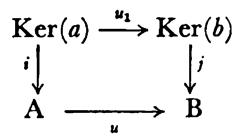
\includegraphics[keepaspectratio]{images/part001_d47c3bb2.jpg}}

\begin{enumerate}
\def\labelenumi{(\arabic{enumi})}
\setcounter{enumi}{14}
\tightlist
\item
\end{enumerate}

\pandocbounded{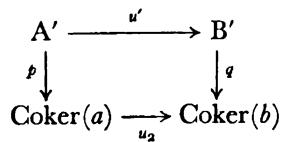
\includegraphics[keepaspectratio]{images/part001_9d56bddd.jpg}}

are commutative, \(i\) and \(j\) denoting the canonical injections and \(p\) and \(q\) the canonical surjections.

If \(x \in \operatorname{Ker}(a)\) , then \(a(x) = 0\) and \(b(u(x)) = u'(a(x)) = 0\) , hence \(u(x) \in \operatorname{Ker}(b)\) , and the existence and uniqueness of \(u_1\) are then immediate. Similarly, we have \(u'(a(A)) = b(u(A)) \subset b(B)\) , then by taking quotients \(u'\) gives a homomorphism \(u_2\) : \(\operatorname{Coker}(a) \to \operatorname{Coker}(b)\) , which is the only homomorphism for which (15) is commutative.

Let us now start with the commutative diagram (10) of commutative groups; there corresponds to it by Lemma 1 a diagram

\begin{enumerate}
\def\labelenumi{(\arabic{enumi})}
\setcounter{enumi}{15}
\tightlist
\item
\end{enumerate}

\pandocbounded{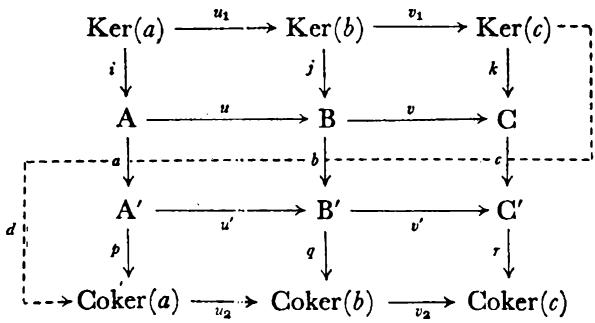
\includegraphics[keepaspectratio]{images/part001_af6ee28a.jpg}}

where \(i, j, k\) are the canonical injections, \(p, q, r\) the canonical surjections and \(u_{1}, u_{2}\) (resp. \(v_{1}, v_{2}\) ) the homomorphisms canonically associated with \(u, u'\) (resp. \(v, v'\) ) by Lemma 1. It is immediately verified that this diagram is commutative.

PROPOSITION 2. Suppose that in the commutative diagram (10) the sequences \((u, v)\) and \((u', v')\) are exact. Then:

\begin{enumerate}
\def\labelenumi{(\roman{enumi})}
\item
  \(v_{1} \circ u_{1} = 0\) ; if \(u'\) is injective, the sequence \((u_{1}, v_{1})\) is exact.
\item
  \(v_{2} \circ u_{2} = 0\) ; if \(v\) is surjective, the sequence \((u_{2}, v_{2})\) is exact.
\item
  Suppose that \(u'\) is injective and \(v\) is surjective. Then there exists one and only one homomorphism \(d: \operatorname{Ker}(c) \to \operatorname{Coker}(a)\) with the following property: if \(x \in \operatorname{Ker}(c)\) , \(y \in B\) and \(t' \in A'\) satisfy the relations \(v(y) = k(x)\) and \(u'(t') = b(y)\) , then \(d(x) = p(t')\) . Moreover the sequence
\end{enumerate}

\[
(*) \quad \operatorname{Ker} (a) \xrightarrow {u _ {1}} \operatorname{Ker} (b) \xrightarrow {v _ {1}} \operatorname{Ker} (c) \xrightarrow {d}
\]

\[
\operatorname{Coker} (a) \xrightarrow {u _ {2}} \operatorname{Coker} (b) \xrightarrow {v _ {2}} \operatorname{Coker} (c)
\]

is exact.

Let us prove (i). As \(u_{1}\) and \(v_{1}\) have the same graphs as the restrictions of \(u\) and \(v\) to \(\operatorname{Ker}(a)\) and \(\operatorname{Ker}(b)\) respectively, we have \(v_{1} \circ u_{1} = 0\) . Then

\[
\operatorname{Ker} (v _ {1}) = \operatorname{Ker} (b) \cap \operatorname{Ker} (v) = \operatorname{Ker} (b) \cap \operatorname{Im} (u) = \operatorname{Im} (j) \cap \operatorname{Im} (u).
\]

But, by Proposition 1, (i), \(\operatorname{Ker}(v_1) = \operatorname{Im}(j \circ u_1) = \operatorname{Im}(u_1)\) if \(u'\) is injective.

Let us prove (ii). As \(u_{2}\) and \(v_{2}\) are obtained from \(u\) and \(v\) by taking quotients, it is clear that \(v_{2} \circ u_{2} = 0\) . Suppose that \(v\) is surjective; as \(q\) and \(p\) are surjective, it follows from the hypotheses and Proposition 1, (ii) that

\[
\begin{array}{r l} \operatorname{Ker} (v _ {2}) & = q (\operatorname{Ker} (v _ {2} \circ q)) = q (\operatorname{Ker} (v ^ {\prime}) + \operatorname{Im} (b)) = q (\operatorname{Ker} (v ^ {\prime})) = q (\operatorname{Im} (u ^ {\prime})) \\ & = \operatorname{Im} (q \circ u ^ {\prime}) = \operatorname{Im} (u _ {2} \circ p) = \operatorname{Im} (u _ {2}). \end{array}
\]

Finally let us prove (iii). For \(x \in \operatorname{Ker}(c)\) there exists \(y \in B\) such that \(v(y) = k(x)\) since \(v\) is surjective; moreover \(v'(b(y)) = c(k(x)) = 0\) and consequently there exists a unique \(t' \in A'\) such that \(u'(t') = b(y)\) , since \(u'\) is injective. We now show that the element \(p(t') \in \operatorname{Coker}(a)\) is independent of the element \(y \in B\) such that \(v(y) = k(x)\) . For if \(y' \in B\) is another element such that \(v(y') = k(x)\) , then \(y' = y + u(z)\) , where \(z \in A\) ; we show that if \(t'' \in A'\) is such that \(u'(t'') = b(y')\) then \(t'' = t' + a(z)\) ; for

\[
u ^ {\prime} \left(t ^ {\prime} + a (z)\right) = u ^ {\prime} \left(t ^ {\prime}\right) + u ^ {\prime} (a (z)) = b (y) + b (u (z)) = b (y + u (z)) = b \left(y ^ {\prime}\right).
\]

Finally, it follows that \(p(t'') = p(t') + p(a(z)) = p(t')\) . Then it is possible to set \(d(x) = p(t')\) and the mapping \(d: \operatorname{Ker}(c) \to \operatorname{Coker}(a)\) has thus been defined. If now \(x_1, x_2\) are elements of \(\operatorname{Ker}(c)\) and \(x = x_1 + x_2\) , we take elements \(y_1, y_2\) of B such that \(v(y_1) = k(x_1)\) and \(v(y_2) = k(x_2)\) and choose for \(y \in B\) the element \(y_1 + y_2\) ; it is then immediate that \(d(x) = d(x_1) + d(x_2)\) and hence \(d\) is a homomorphism.

Suppose that \(x = v_{1}(x')\) for some \(x' \in \operatorname{Ker}(b)\) ; then take \(y \in B\) to be the element \(j(x')\) . As \(b(j(x')) = 0\) , it follows that \(d(x) = 0\) , hence \(d \circ v_{1} = 0\) . Conversely, suppose that \(d(x) = 0\) . In the above notation we then have \(t' = a(s)\) , where \(s \in A\) . In this case we have \(b(y) = u'(t') = u'(a(s)) = b(u(s))\) , or \(b(y - u(s)) = 0\) . The element \(y - u(s)\) is therefore of the form \(j(n)\) , where \(n \in \operatorname{Ker}(b)\) , and we have \(k(x) = v(y) = v(u(s) + j(n)) = v(j(n)) = k(v_1(n))\) ; as \(k\) is injective, \(x = v_1(n)\) , which proves that the sequence (*) is exact at \(\operatorname{Ker}(c)\) .

Finally, we have (always in the same notation)

\[
u _ {2} (d (x)) = u _ {2} \left(p \left(t ^ {\prime}\right)\right) = q \left(u ^ {\prime} \left(t ^ {\prime}\right)\right) = q (b (y)) = 0
\]

and hence \(u_2 \circ d = 0\) . Conversely, suppose that an element \(w = p(t')\) of Coker(a) is such that \(u_2(w) = u_2(p(t')) = 0\) (where \(t' \in A'\) ). Then \(q(u'(t')) = 0\) and consequently \(u'(t') = b(y)\) for some \(y \in B\) ; as \(v'(u'(t')) = 0\) , we have \(v'(b(y)) = 0\) , hence \(c(v(y)) = 0\) , in other words \(v(y) = k(x)\) for some \(x \in \operatorname{Ker}(c)\) , and by definition \(w = d(x)\) , which shows that the sequence (*) is exact at

Coker(a). It has been seen in (i) that it is exact at \(\operatorname{Ker}(b)\) and in (ii) it is exact at \(\operatorname{Coker}(b)\) , which completes the proof of (iii).

Remark. If the groups of the diagram (10) are all (for example, right) modules over a ring \(\Lambda\) and the homomorphisms are \(\Lambda\) -module homomorphisms, it is soon verified that the homomorphism \(d\) defined in Proposition 2, (iii) is also a \(\Lambda\) -module homomorphism: if \(x \in \operatorname{Ker}(c)\) and \(\alpha \in \Lambda\) , and \(y \in B\) is such that \(v(y) = k(x)\) , it is sufficient to note that \(v(y\alpha) = k(x\alpha)\) .

COROLLARY 1. Suppose that the diagram (10) is commutative and the two rows are exact. Then:

\begin{enumerate}
\def\labelenumi{(\roman{enumi})}
\item
  If \(u'\) , \(a\) and \(c\) are injective, \(b\) is injective.
\item
  If \(v, a\) and \(c\) are surjective, \(b\) is surjective.
\end{enumerate}

Assertion (i) is a consequence of assertion (i) of Proposition 2: for \(\operatorname{Ker}(a) = 0\) and \(\operatorname{Ker}(c) = 0\) , hence \(\operatorname{Ker}(b) = 0\) .

Assertion (ii) is a consequence of assertion (ii) of Proposition 2: for \(\operatorname{Coker}(a) = 0\) and \(\operatorname{Coker}(c) = 0\) , hence \(\operatorname{Coker}(b) = 0\) .

COROLLARY 2. Suppose that the diagram (10) is commutative and the two rows are exact. Under these conditions:

\begin{enumerate}
\def\labelenumi{(\roman{enumi})}
\item
  If \(b\) is injective and if \(a\) and \(v\) are surjective, then \(c\) is injective.
\item
  If \(b\) is surjective and if \(c\) and \(u'\) are injective, then \(a\) is surjective.
\end{enumerate}

To prove (i) consider the diagram

\[
\begin{array}{c c c} u (\mathrm{A}) & \xrightarrow {w} \mathrm{B} & \xrightarrow {v} \mathrm{C} \\ a ^ {\prime} \Big \downarrow & b \Big \downarrow & c \Big \downarrow \\ u ^ {\prime} (\mathrm{A} ^ {\prime}) & \xrightarrow [ w ^ {\prime} ]{} \mathrm{B} ^ {\prime} & \xrightarrow [ v ^ {\prime} ]{} \mathrm{C} ^ {\prime} \end{array}
\]

where \(a'\) is the mapping with the same graph as the restriction of b to \(u(\mathbf{A})\) and w and \(w'\) are the canonical injections; clearly this diagram is commutative and its rows exact. Moreover \(w'\) is injective and by hypothesis v is surjective; then by Proposition 2, (iii) we have an exact sequence

\[
0 = \operatorname{Ker} (b) \longrightarrow \operatorname{Ker} (c) \stackrel {d} {\longrightarrow} \operatorname{Coker} (a ^ {\prime}) = 0
\]

since \(b\) is injective and \(a'\) is surjective; whence \(\operatorname{Ker}(c) = 0\) .

To prove (ii) consider the diagram

\[
\begin{array}{c} \mathrm{A} \xrightarrow {u} \mathrm{B} \xrightarrow {w} v (\mathrm{B}) \\ a ^ {\prime} \Biggl \downarrow \qquad \qquad b \Biggl \downarrow \qquad \qquad c ^ {\prime} \Biggl \downarrow \\ \mathrm{A} ^ {\prime} \xrightarrow [ w ^ {\prime} ]{} \mathrm{B} ^ {\prime} \xrightarrow [ v ^ {\prime} ]{} v ^ {\prime} (\mathrm{B} ^ {\prime}) \end{array}
\]

where this time \(c'\) is the mapping with the same graph as the restriction of c to \(v(\mathbf{B})\) and \(w\) and \(w'\) have respectively the same graphs as \(v\) and \(v'\) ; this diagram is commutative and its rows exact. Moreover \(w\) is surjective and by hypothesis \(u'\) is injective; then by Proposition 2, (iii) we have an exact sequence

\[
0 = \operatorname{Ker} (c ^ {\prime}) \xrightarrow {d} \operatorname{Coker} (a) \longrightarrow \operatorname{Coker} (b) = 0
\]

since \(b\) is surjective and \(c'\) is injective; whence Coker \((a) = 0\) .

